% This is a sample for the annual report.  The following things are 
% not standard tex, because of numbering conventions, layout, etc.
%
% PLEASE READ THE FOLLOWING, SPECIFICALLY THE PART ABOUT SPECIAL COMMANDS FOR REFERENCING TABLES AND FIGURES
%
% Do not typeset this LaTex file directly, instead use MakeArticle.tex.
% To typeset, the following files must be in located the same folder:  
%
% preamble2016.tex
% examplefig.eps
% ExampleArticle.tex
% MakeArticle.tex
%
% preamble2016.tex adds the \begin{document} command and defines CENPA specific formatting.
% It also defines the MACRO \auth{} which will format the authors.
%
% 1) Titles must be built as in the example.  Use \section{}, \subsection{}, \subsubsection{},  or \paragraph{}.
%
% 2) Authors go below title, use the \auth{} MACRO as shown in the example. Author footnotes should be done as 
% in the example with Van~Schagen.  The command \, makes a nice space between initials.
%
% 3) Footnotes in the text should be done with the \footnoteText{} command.
% The format for references to journals is shown. Also shown is the reference
% to old annual reports using \CENPAfoot{year}{page}
%
% 4) Figures should be done with the graphicx package (note X not S at the end)
% Use .eps, .pdf, .png, or .jpg files, please
% If you need to put two figures side by side and don't know how, see me.
%
% 5) If you want a table with no reference or caption, just put it in.
%
% 6) Every article must have a label.  Put a \label{} within the title (\subsection{}) as shown below. To reference 
% another article in this report use the \secref{} MACRO to refer to it from the other article. \secref{} will return
% (see Sec. W.X) or (see Sec. W.X.Y) or (see Sec. W.X.Y.Z) depending on the nesting. The parentheses WILL be there.
%
% Figures and tables also use your article label for the numbering scheme.
%
% Use the MACRO \figcaption{articlelabel}{figurecaption} to make the figure caption at any section level.  
% The argument is the text of the figure caption.
% Use the MACRO \figref{articlelabel}{figurelabel} to reference figures at the any section level. The argument is the figure label.
%
% Use the MACRO \tabcaption{articlelabel}{tablecaption} to make the table caption at the subsection level. 
% The argument is the text of the table caption.
% Use the MACRO \tabref{articlelabel}{tablelabel} to reference the tables at any section level. The argument is the table label.
%
% Label your figure or table with something likely to be unique to the annual report.  
% Everybody will have a "figure1" so use something descriptive.  E.g. He6YieldVsBeamCurrent.
%
% The MACRO \degrees makes a degree symbol that looks right
% The MACRO \cpp produces a C++ that looks right
% \iso{13}{N} makes an isotope
% \MJ\ makes small cap Majorana with a trailing space. 
% \MJ makes small cap Majorana without a space. 
% \snop makes a nice representation of SNO+
% \MJDemo Makes the small cap version of Demonstrator
% \nonubb makes neutrinoless double beta decay in math mode
% \gp makes mathmode g sub cap P
% \LS makes mathmode cap Lambda sub cap S
% \RD makes mathmode cap Lambda sub cap D
%
%
%
\subsection{The \iso{4}{He}(\boldmath $\alpha , \gamma $\unboldmath)\iso{8}{Be} experiment \label{articlelabel} }
%
% Please make multi-word titles with the first capitalized only: e.g. \subsection{A title with multiple words about Coulomb's law}
% You naturally capitalize things which would be capitalized in a normal sentence. Note that there is a label for this title. Also note
% the examples of the use of the \iso{}{} MACRO and that it uses the \boldmath MACRO for producing normal text in the TOC and
% bold mathmode in the title.
%
% In this example, \subsection is used as the starting level. Other valid hierarchal constructs are \section, \subsubsection and \paragraph.
% Unless otherwise instructed,  it is safe to leave the document level at \subsection{} when you submit your titles and articles.  
%
\auth{
R.~Hazama, 
K.\,A.~Snover, 
\underline{D.\,W.~Storm},
J.\,P.\,S.~Van~Schagen\footnoteAuthor[1]{Presently at WRQ, Seattle, 98109.}, 
D.\,D.~Victory\footnotemarkAuthor[1], 
and
Z.\,Z.~Zootsuit\footnoteAuthor[2]{Cracker Institute, Crackerville, USA.}
}
% Notice the repeated footnote format for \footnoteAuthor[1]{argument} and footnotemarkAuthor[1]. This author list is
% alphabetized by last name, fully initialed, correctly formatted, and very easy to read.

% Do not indent the first paragraph of each article

\noindent     % This prevents the indentation of the first paragraph. Don't skip the next line.
We are in the process of completing the analysis of the 
high-precision measurement\CENPAfoot{1999}{5} (that's a CENPA annual report footnote, by the way)
of the \iso{4}{He}($\alpha , \gamma$)\iso{8}{Be}
reaction.   We are using the results of Marrs {\it et al}\,\footnoteText{\label{marrs}R.\,E.~Marrs, E.\,G.~Adelberger, and K.\,A.~Snover, Phys. Rev.  C {\bf 16}, 61 (1977).}. %I'm really smart. I just footnoted italicized text so I needed to add a clever little space using \,. Can you see that trick?
I can repeat that last footnote because it's labeled. Isn't that handy? See how this paragraph is not indented? Then you write more text and so on. Try to make it interesting and spell stuff right.

As you can see, this paragraph is indented, while the first one wasn't.
I'm going to use that last footnote again\footref{marrs} like that. Is that easy, or what? The footnotes are renumbered on a per page basis. Some interesting results are given in \tabref{articlelabel}{mytable}. Look at the table this produces. See how it is numbered and captioned.

\begin{table}[h]
\begin{center}
\begin{tabular}{lcr}
Day of week &  hours of sun & hours of rain \\
Monday &	1	& 3 \\
Tuesday & 5  & 7 \\
Friday & 9 & 0 \\
\end{tabular}

\tabcaption{articlelabel}{~~~Local weather conditions for the week of February 35.}
\label{mytable}  %put label{} after \tabcaption{}

\end{center}
\end{table}

And what do you think of \figref{articlelabel}{myFig1}?
Note the figure number and caption are done in an unusual way to enable the numbering to
follow the section numbering.  Be sure that you copy this numbering scheme, substituting only your
own figure and table labels for the last bit.

\begin{figure}[h]

\hfil  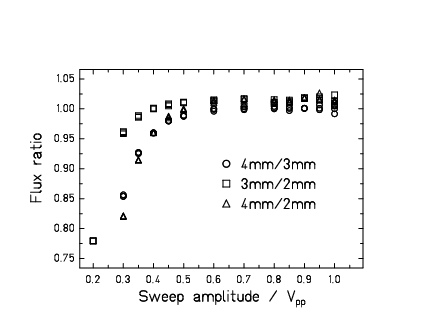
\includegraphics[width=.45\textwidth]{examplefig} \hfil 
% the following blank line is important

\figcaption{articlelabel}{Ratio of beam fluxes through different size apertures, measured with a deuteron beam ($E_d$ = 770 keV).}

\label{myFig1}  %put label{} after \figcaption{}

\end{figure}

Now, for some silly reason, I'm going to reproduce the first table in \tabref{articlelabel}{mytable2} where it is repeated exactly. That's a dumb idea. Why repeat the same table twice? Don't do it in your article, you'll come across as a bonehead. Instead, write smart and clever stuff that will captivate people. This is just an example.

\begin{table}[h]
\begin{center}
\begin{tabular}{lcr}
Day of week &  hours of sun & hours of rain \\
Monday &	1	& 3 \\
Tuesday & 5  & 7 \\
Friday & 9 & 0 \\
\end{tabular}

\tabcaption{articlelabel}{The same local weather conditions again for the week of February 35.}
\label{mytable2} %put label{} after \tabcaption{}

\end{center}
\end{table}



Nobody wrote any \cpp code.  See how weird C++ is typeset? There are MACROs for oddball stuff like \MJ\ and for \snop\ as well. There is one to make \MJ\ end with a period like \MJ. Do you want to typeset 20 degrees~C? Here's how: 20\degrees~C.

Lets write another paragraph to fill up some space.  Back in the old days we did this Annual Report with a typewriter.  {\tt Typewriters look like this. } Need an old annual report footnote?  Here is how\CENPAfoot{1923}{6}. See how the footnotes renumbered to 1 on this new page?


